\documentclass[10pt]{article}

\usepackage[margin=0.65in]{geometry}
\usepackage{graphicx}
\usepackage{xcolor}
\usepackage{hyperref}
\usepackage{enumitem}
\usepackage{titlesec}

\definecolor{asuMaroon}{HTML}{8C1D40}
\definecolor{textGray}{HTML}{4B5563}

\hypersetup{
  colorlinks=true,
  urlcolor=asuMaroon,
  linkcolor=asuMaroon
}

\setlength{\parindent}{0pt}
\setlength{\parskip}{4pt}
\setlist[itemize]{leftmargin=1.2em, itemsep=2pt, topsep=2pt}
\setlist[enumerate]{leftmargin=1.5em, itemsep=3pt, topsep=3pt}
\titleformat{\section}{\large\bfseries\color{asuMaroon}}{}{0pt}{}

\begin{document}

{\Large\bfseries DIT Ion Migration Calculator Quick Start}

\textcolor{textGray}{A concise guide for accessing the public web calculator, uploading DIT data, reviewing the plot, and exporting results.}

\section{Access}

Open the calculator in any modern browser:

\href{https://flabio121.github.io/ion-migration-dit-calculator/}{https://flabio121.github.io/ion-migration-dit-calculator/}

The calculator runs in the browser. Uploaded files are processed locally on the user's computer.

\begin{center}
  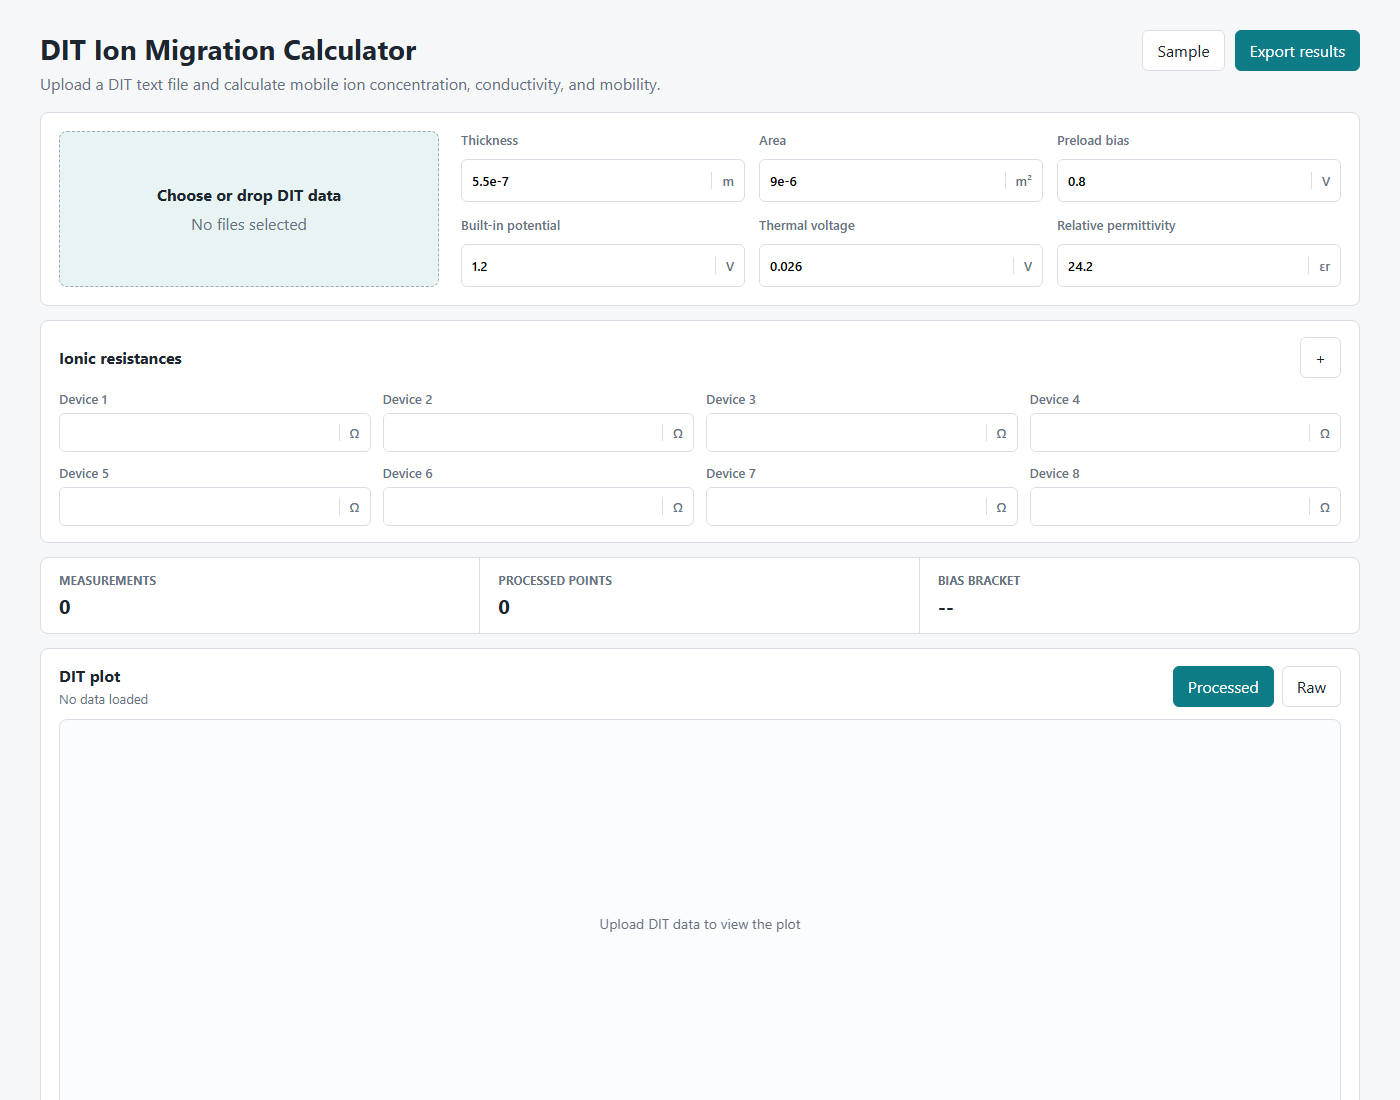
\includegraphics[width=0.92\linewidth]{assets/dit-calculator-home.png}
\end{center}

\section{Before You Start}

Prepare one or more DIT text files. The current calculator expects paired time/current data exported in the same format used by the validated workflow. Have these values ready if needed:

\begin{itemize}
  \item Device thickness and active area.
  \item Preload bias, built-in potential, thermal voltage, and relative permittivity.
  \item Optional ionic resistance values for conductivity and mobility.
\end{itemize}

\section{Use The Calculator}

\begin{enumerate}
  \item Open the website and drag one or more \texttt{.txt} files into the upload area, or click the upload area to select files.
  \item Confirm the device constants. Defaults are pre-filled, but should be changed if the device geometry or assumptions differ.
  \item Enter ionic resistance values when conductivity and mobility are needed. Leave them blank if only concentration is required.
  \item Inspect the DIT plot. Use \textbf{Processed} to see the trace used for integration and \textbf{Raw} to check the imported data.
  \item Review the result table. Key outputs include integrated charge, concentration in \(\mathrm{cm^{-3}}\), conductivity, mobility, and data-point count.
  \item Click \textbf{Export results} to download the summary table as a CSV file.
\end{enumerate}

\section{Notes}

\begin{itemize}
  \item Results depend strongly on active area, thickness, voltage assumptions, and the processed integration window.
  \item Conductivity and mobility require ionic resistance inputs; concentration does not.
  \item For reproducibility, keep the uploaded raw data, exported CSV, and device constants with the experiment record.
\end{itemize}

\end{document}
